\section{Gestione degli errori nello strato fisico}

    Ci siamo occupati della trasmissione dei dati e della loro natura. Durante la comunicazione all'interno di una rete, per vari motivi, il messaggio può subire delle alterazioni: questo fenomeno è detto \textbf{errore di trasmissione}. 
    
    A seconda del tipo di di rete si profilano vari scenari: alcuni applicativi continuano a funzionare anche in presenze di errori, altre che ne richiedono il rilevamento ma non la correzione, e altre ancora che necessitano imperativamente che gli errori siano corretti prima di ripristinare il funzionamento della trasmissione.
    
    \vspace{3mm}
    
    L'aspetto più interessante è capire quando si verifica un errore di trasmissione.
    
    Se immaginiamo i dati come flussi di bit, possiamo distinguere due tipi di errori:
    
    \begin{itemize}
        \item \textbf{Errore singolo}, quando un bit 0 viene cambiato in 1 e viceversa
        \item \textbf{Errore multiplo}, quando più bit vengono interpretati erroneamente
    \end{itemize}
    
    Il rilevamento e la correzione degli errori vengono svolti impiegando la \textbf{tecnica della ridondanza}.
    
    La ridondanza richiama il concetto di dati aggiuntivi: per capire se si sono verificati degli errori, all'invio del messaggio posso aggreggare a quest'ultimo dei \textit{bit di controllo} che, lato destinatario, vengono interpretati per capire o meno se ci sono stati errori.
    
    \vspace{3mm}
    
    Ci sono varie tecniche di aggiungere bit di controllo (detti anche \textit{bit ridondanti}) ad un messaggio: questo processo si chiama codifica. In letteratura, spiccano la \textit{codifica a blocchi} e la \textit{codifica convulazionale}.
    
    \begin{center}
        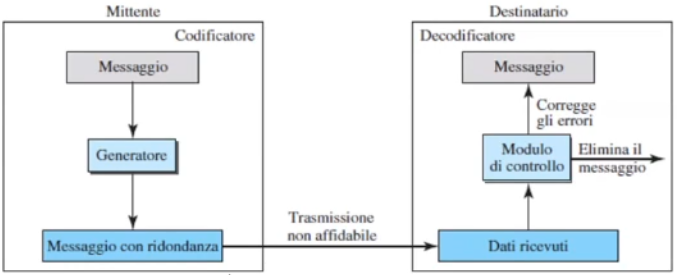
\includegraphics[scale=0.5]{images/Esempio-Codifica.png}
    \end{center}
    
    \subsection{Codifica a blocchi}
        
        La \textbf{codifica a blocchi} prevede che i dati vengono divisi in blocchi, ognuno di $k$ bit. I blocchi prendono il nome di \textit{parole sorgente}.
        
        Per ogni parola sorgente vengono aggiunti $r$ bit ridondanti. Risulta che la lunghezza dell'i-esima parola sorgente, rinominata in \textit{parola codice}, sarà $n=r+k$. La parola codice è il messaggio che viene effettivamente inviato sul canale trasmissivo.
        
        Dato un insieme di blocchi di dimensione $k$, si possono ottenere al più $2^k$ parole sorgenti. Analogamente, si possono ottenere al più $2^n$ parole codice.
        
        \vspace{3mm}
        
        Ogni tecnica di codifica a blocchi può rilevare solo un certo numero di errori. Il numero di errori rilevabili dipesa dalla progettazione del codice a blocchi stesso; tuttavia, un numero elevato di errori può causare una decodifica errata. La maggior parte delle tecniche di codifica a blocchi si basa sulla \textit{distanza di Hamming}.
        
        \vspace{3mm}
        
        La distanza di Hamming $d(x,y)$ tra due parole $x$ e $y$ (della stessa lunghezza) è il numero di differenza fra i bit della stessa posizione, calcolabile con $x XOR y$ e contando il numero di bit 1 nel risultato.
        
        La distanza minima di Hamming all'interno di una codifica è la distanza di Hamming minima fra ogni coppia di parole codice. Le performance di uno schema di codifica a blocchi, in termini di correzione e rilevazione degli errori, dipende proprio dalla distanza minima di Hamming, tramite la quale si producono i due seguenti risultati.
        
        \vspace{3mm}
        
        Per garantire il rilevamento di un numero di errori minimo o uguale a $s$, occorre un codice con distanza minima di Hamming $d_min >= s+1$.
        
        Per garantire la correzione fino a $t$ errori, occorre un codice con distanza minima di Hamming $d_min >= 2t+1$.
        
        \vspace{3mm}
        
        Diamo un'occhiata, adesso, al tipo più importante di codifica a blocchi: il codice lineare.
        
        \subsubsection{Codice lineare}
        
            Se valuto le parole codice di un codice a blocchi, ed eseguo lo $XOR$ fra due parole codice qualsiasi, ottengo una parola codice valida. In termini pratici, esiste una proprietà di chiusura rispetto allo $XOR$ delle parole codice. Quando il codice a blocchi gode di questa proprietà, si parla di \textbf{codici lineari}.
            
            I codici lineari si distinguono in \textbf{codici a priorità}, \textbf{codici di Hamming} e \textbf{codici ciclici}.
            
            \subsubsubsection{Codice a parità}
            
                I codici a parità sono caratterizzati da una semplice proprietà: si aggiunge un solo bit di ridondanza, detto bit di parità. Da parole sorgente di lunghezza $k$, si ottengono parole codice di $n=k+1$ bit.
                
                Data la parola sorgente, per determinare se aggiungere come bit di parità 0 o 1, ci si prefissa di ottenere, tramite la sequenza di 1 nel flusso di bit, un numero pari.
                
            \subsubsubsection{Codice di Hamming}
            
                I codici di Hamming si denotano con $C(n, k)$, dove $n$ è la lunghezza delle parole codice, e $k$ è la lunghezza delle parole sorgente.
                
                Per i codici di Hamming si aggiungono 3 o più bit ridondanti $m$, grazie a osservazioni empiriche. Questa scelta porta una serie di vantaggi nel calcolo della \textit{sindrome della codifica}.
                
                \vspace{3mm}
                
                Per $m=3$, si desidera $C(7,4)$.
                
                Per $m>=3$, $n=2^m - 1$ e $k=n-m$. Risulterà $r=m$.
                
                \vspace{3mm}
                
                Le parole codice nella codifca di Hamming si basano su un meccanismo di combinazione lineare dei bit a disposizione. Ad esempio, data una parola sorgente di 4 bit, si aggiungono arbitrariamente 3 bit ridondanti. La lunghezza della parola codice sarà 7. Vi sono $2^7$ parole codici possibili, di cui $2^4$ parole codici valide.
                
                Posti $r_1, r_2, r_3$ i bit ridondanti e $a_0, a_1, a_2, a_3$ bit della parola sorgente, risulterà che $r_1 = a_2 + a_1 + a_0$, $r_2 = a_3 + a_2 + a_1$ e $r_3 = a_3 + a_1 + a_0$.
                
                \vspace{3mm}
                
                Al destinatario arriveranno 7 bit, il quale si calcolerà la sindrome della codifica. La sindrome è costituita da $m$ bit che si usano per verificare se il messaggio è arrivato correttamente. Si usa la medesima combinazione lineare dei bit ridondanti, sommando i bit associati ricevuti dal d. Se la sindrome è diversa da (0, 0, 0), dove ogni elemento della tupla è l'm-esimo bit ridondante estrapolato dal destinatario risultano errori.
                
                \vspace{3mm}
                
                Data una generica tabella con parole sorgente e parola codice, si calcola la distanza minima di Hamming per determinare quanti errori si possono rilevare e correggere.
                
            \subsubsubsection{Codice ciclico}
            
                Un codice è lineare se vi è una chiusura rispetto allo $XOR$. Nei codici ciclici vi è un'ulteriore chiusura rispetto allo \textit{shift ciclico}.
                
                Ad esempio, se $101101$ è una parola codice, anche $110110$ lo è.
                
                Per costruire una parola codice a partire da una parola sorgente, si utilizza un divisore. Il divisore viene usato, appunto, per dividere la parola sorgente (opportunamente allungata) per ottenere i bit ridondanti. In termini pratici, il modulo di codifica prende in input una parola sorgente e la allunga con $n-k$ bit con valore 0. 
                
                Le seguenti immagini illustrano il processo di codifica e decodifica.
                
                \begin{center}
                    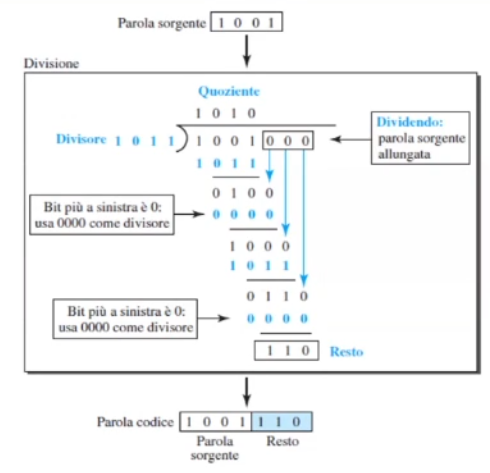
\includegraphics[scale=0.5]{images/Codici-Ciclici.png}
                \end{center}
                
                \begin{center}
                    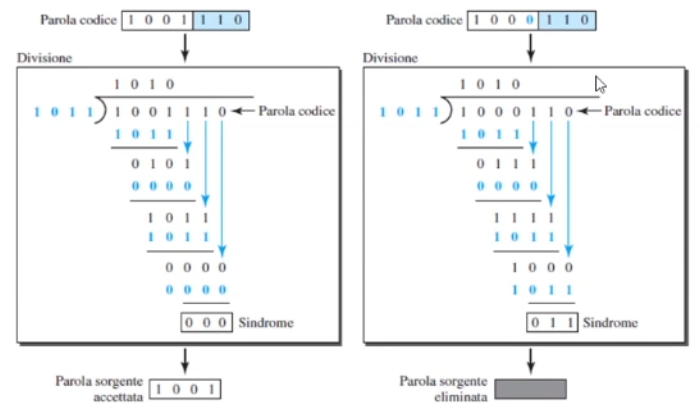
\includegraphics[scale=0.5]{images/Codici-Ciclici-Decodifica.png}
                \end{center}
                
    \subsection{Somme di controllo}
    
        Le \textbf{somme di controllo} sono un meccanismo per il rilevamento di errori. I bit inviati possono essere mappati come una sequenza di numeri, alla fine della quale se ne appende la somma. Se tale somma di destinazione coinciderà con quella di invio, allora non si sarà verificato alcun errore.
        
        Per facilitare il controllo, si può spedire il negativo della somma: al ricevitore, in questo modo, basterà effettuare la somma di tutti i numeri, che in caso di assenza di errori dovrà coincidere con 0.
        
        Il problema della somma di controllo è che potrebbe essere un numero molto grande se gli addendi sono numerosi.
                